


\end{enumerate}

\begin{figure}[htb]
\begin{center}
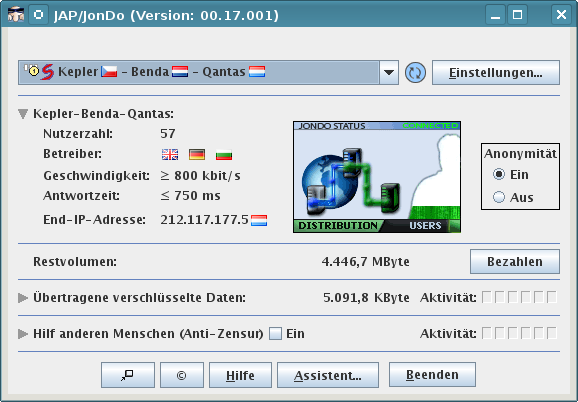
\includegraphics[scale=0.75]{../screenshots/jap-java.png}
\caption{Hauptfenster von JonDo}
\label{abb:jap_haupt}
\end{center}
\end{figure}

Startet man JonDo, �ffnet sich das im Bild \ref{abb:jap_haupt} gezeigte Hauptfenster des Programms. Hier kann man eine Kaskade ausw�hlen und mit Klick auf die Option \textit{Anonymit�t Ein} die Verbindung herstellen.\\

\subsection{JonDonym Premium Account einrichten}
JonDonym ist ein kommerzieller Dienst, der nicht von Finanzierungen durch Regierungen abh�ngig ist. Die Einnahmen der Premium-Nutzer bilden Hauptteil der Finanzierung und erm�glichen damit einen von Regierungsinteressen unabh�ngigen Anonymisierungsdienst.\\

Die Premium-Dienste von JonDonym bieten folgende Vorteile: 
\begin{itemize}
 \item 20x h�here Geschwindigkeit (siehe: Status der Mix-Server)
 \item Keine Begrenzung der Dateigr��e f�r Downloads auf 2 MB.
 \item Alle Internet-Protokolle nutzbar (kostenfreie Kaskaden nur f�r Surfen)
 \item SOCKS5 Support f�r Anwendungen, die keinen HTTP-Proxy kennen
 \item Hohe Verf�gbarkeit (kostenfreie Kaskaden sind h�ufig �berlastet)
 \item In der Regel wird der Datenverkehr durch 3 L�nder geleitet.
 \item Zugriff auf den anonymen Dateispeicher von JonDonym unter \href{https://storage.anonymous-proxy-servers.net}{https://storage.anonymous-proxy-servers.net}
\end{itemize}

Am einfachsten ist es, wenn man im \textbf{Webshop der JonDos GmbH} \footnote{ \href{https://shop.anonymous-proxy-servers.net/bin/payment}{https://shop.anonymous-proxy-servers.net/bin/payment}} einen Premium Coupon kauft und mit Paysafecard bezahlt (siehe: \textit{Bezahlen im Netz}). Die Tarife von JonDonym sind auf die angebotenen Paysafecard Gutscheine abgestimmt, so dass man f�r alle Tarife passende Gutscheine kaufen kann.\\

Im ersten Schritt w�hlt man den Tarif und akzeptiert die AGB:

\begin{center}
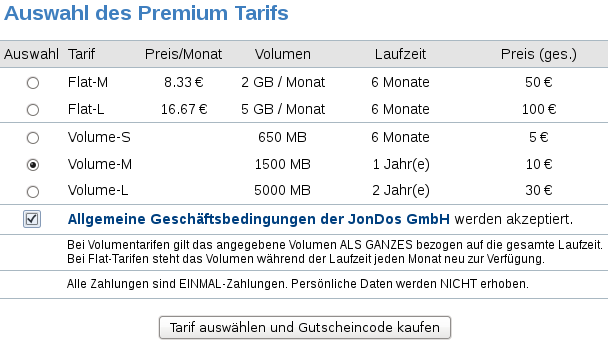
\includegraphics[scale=0.75]{../screenshots/jondo-premium-web1.png}
\end{center}

Im zweiten Schritt kann man die Bezahlmethode w�hlen.

\begin{center}
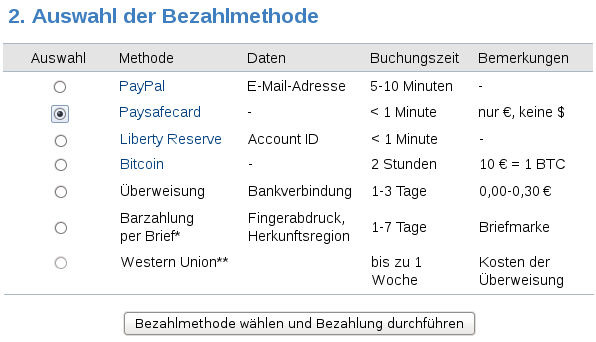
\includegraphics[scale=0.75]{../screenshots/jondo-premium-web2.png}
\end{center}

Nach der Auswahl von Paysafecard wird man auf die Webseite von Paysafecard weitergeleitet, gibt dort den Gutscheincode ein und erh�lt dann auf der Webseite von JonDos einen Premium Code (wenn Paysafecard den Gutschein akzeptiert hat).

\begin{center}

\includegraphics[scale=0.75]{../screenshots/jondo-premium-web4.png}
\end{center}

Mit dem Code kann man im JonDo ein Konto erstellen. Im Hauptfenster klickt man auf den Button \textit{Bezahlen}. Es startet ein Assistent, der durch die Einrichtung des Kontos f�hrt. Den Premium Code kann man im ersten Schritt eingeben - fertig. Zuk�nftig kann man im Hauptfenster von JonDo Kaskaden mit 3 Mix-Servern w�hlen, um die Vorteile der Premiumdienste zu genie�en.

\begin{figure}[htb]
\begin{center}
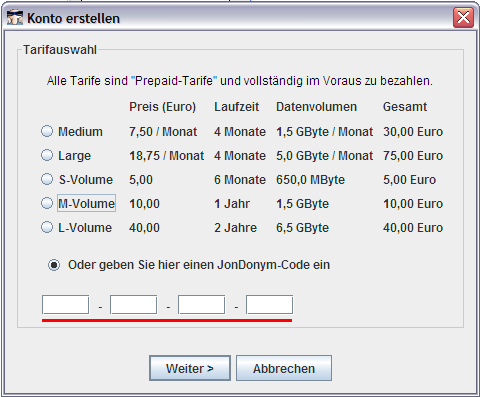
\includegraphics[scale=0.55]{../screenshots/jondo-pay2.png}
\caption{Jondonym Premium Code einl�sen}
\label{abb:jappremium}
\end{center}
\end{figure}
